\documentclass[border=8pt]{standalone}
\usepackage{tikz}
\begin{document}
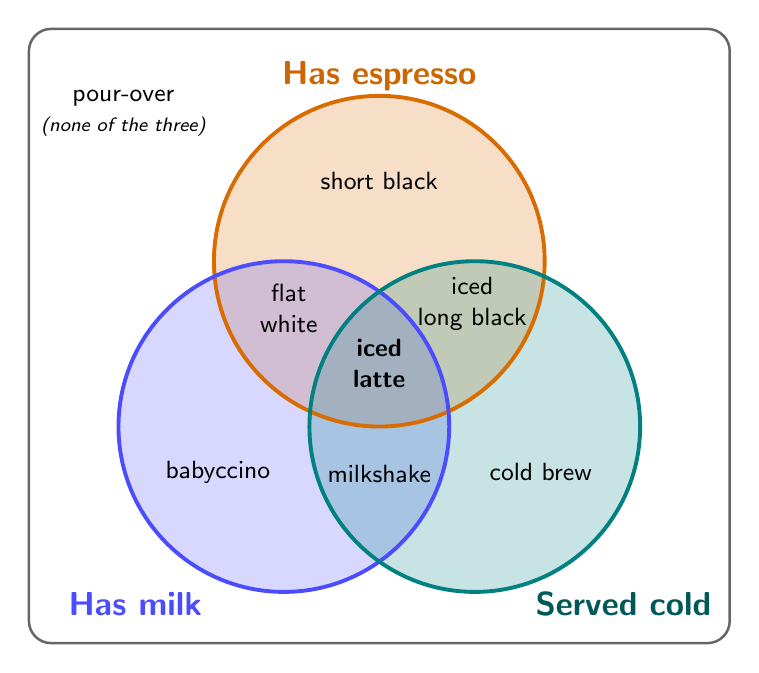
\begin{tikzpicture}

  % ================= geometry =================
  \def\R{2.1}                             % circle radius
  \def\d{1.4}                             % centre offset from origin
  \coordinate (E) at (90:\d);             % Has espresso
  \coordinate (M) at (210:\d);            % Has milk
  \coordinate (C) at (330:\d);            % Served cold

  % ================= universe box =================
  \draw[black!60, line width=0.9pt, rounded corners=8pt]
      (-4.45,-3.45) rectangle (4.45,4.35);

  % ================= circles =================
  \begin{scope}[transparency group]
    \fill[orange!85!black, opacity=0.22] (E) circle (\R);
    \fill[blue!70,         opacity=0.22] (M) circle (\R);
    \fill[teal,            opacity=0.22] (C) circle (\R);
  \end{scope}
  \draw[line width=1.4pt, orange!85!black] (E) circle (\R);
  \draw[line width=1.4pt, blue!70]         (M) circle (\R);
  \draw[line width=1.4pt, teal]            (C) circle (\R);

  % ================= circle captions =================
  \node[font=\sffamily\large\bfseries, text=orange!80!black]  at (0,3.75)    {Has espresso};
  \node[font=\sffamily\large\bfseries, text=blue!70]          at (-3.1,-2.95){Has milk};
  \node[font=\sffamily\large\bfseries, text=teal!70!black]    at (3.1,-2.95) {Served cold};

  % ================= the drinks =================
  % espresso only
  \node[font=\sffamily\small, text=black] at (0,2.42)     {short black};
  % milk only
  \node[font=\sffamily\small, text=black] at (-2.05,-1.28){babyccino};
  % cold only
  \node[font=\sffamily\small, text=black] at (2.05,-1.28) {cold brew};
  % espresso + milk, not cold
  \node[font=\sffamily\small, text=black, align=center] at (-1.15,0.80) {flat\\white};
  % espresso + cold, not milk
  \node[font=\sffamily\small, text=black, align=center] at (1.18,0.86)  {iced\\long black};
  % milk + cold, not espresso
  \node[font=\sffamily\small, text=black] at (0,-1.30)    {milkshake};
  % all three
  \node[font=\sffamily\small\bfseries, text=black, align=center] at (0,0.10) {iced\\latte};
  % none of the three (outside every circle)
  \node[font=\sffamily\small, text=black, align=center] at (-3.25,3.28) {pour-over\\
      {\scriptsize\itshape (none of the three)}}; % outside every circle

\end{tikzpicture}
\end{document}
